%%%%%%%%%%%%%%%%%%%%%%%%%%%%%%%%%%%%%%%%%%%%%%%%%%%%%%%%%%%%%%%%%%%%%%%%
%% Customizações do abnTeX2 (http://abnTeX2.googlecode.com)           %%
%% para a Universidade Estadual do Ceara - UECE                       %%
%%                                                                    %%
%% This work may be distributed and/or modified under the             %% 
%% conditions of the LaTeX Project Public License, either version 1.3 %%
%% of this license or (at your option) any later version.             %%
%% The latest version of this license is in                           %%
%%   http://www.latex-project.org/lppl.txt                            %%
%% and version 1.3 or later is part of all distributions of LaTeX     %%
%% version 2005/12/01 or later.                                       %%
%%                                                                    %%
%% This work has the LPPL maintenance status `maintained'.            %%
%%                                                                    %%
%% The Current Maintainer of this work is Thiago Nascimento           %%
%%                                                                    %%
%% Project available on: https://github.com/thiagodnf/uecetex2        %%
%%                                                                    %%
%% Further information about abnTeX2                                  %%
%% are available on http://abntex2.googlecode.com/                    %%
%%                                                                    %%
%%%%%%%%%%%%%%%%%%%%%%%%%%%%%%%%%%%%%%%%%%%%%%%%%%%%%%%%%%%%%%%%%%%%%%%%

%%%%%%%%%%%%%%%%%%%%%%%%%%%%%%%%%%%%%%%%%%%%%%%%%%%%%%%%%%%%%%%%%%%%%%%%
%% Customizações do abnTeX2 (http://abnTeX2.googlecode.com)           %%
%% para a Universidade Estadual do Ceara - UECE                       %%
%%                                                                    %%
%% This work may be distributed and/or modified under the             %% 
%% conditions of the LaTeX Project Public License, either version 1.3 %%
%% of this license or (at your option) any later version.             %%
%% The latest version of this license is in                           %%
%%   http://www.latex-project.org/lppl.txt                            %%
%% and version 1.3 or later is part of all distributions of LaTeX     %%
%% version 2005/12/01 or later.                                       %%
%%                                                                    %%
%% This work has the LPPL maintenance status `maintained'.            %%
%%                                                                    %%
%% The Current Maintainer of this work is Thiago Nascimento           %%
%%                                                                    %%
%% Project available on: https://github.com/thiagodnf/uecetex2        %%
%%                                                                    %%
%% Further information about abnTeX2                                  %%
%% are available on http://abntex2.googlecode.com/                    %%
%%                                                                    %%
%%%%%%%%%%%%%%%%%%%%%%%%%%%%%%%%%%%%%%%%%%%%%%%%%%%%%%%%%%%%%%%%%%%%%%%%

\documentclass[        
    a4paper,          % Tamanho da folha A4
    12pt,             % Tamanho da fonte 12pt
    chapter=TITLE,    % Todos os capitulos devem ter caixa alta
    section=TITLE,    % Todas as secoes devem ter caixa alta
    oneside,          % Usada para impressao em apenas uma face do papel
    english,          % Hifenizacoes em ingles
    spanish,          % Hifenizacoes em espanhol
    brazil            % Ultimo idioma eh o idioma padrao do documento
]{abntex2}


% Importações de pacotes
\usepackage[utf8]{inputenc}                         % Acentuação direta
\usepackage[T1]{fontenc}                            % Codificação da fonte em 8 bits
\usepackage{graphicx}                               % Inserir figuras
\usepackage{amsfonts, amssymb, amsmath}             % Fonte e símbolos matemáticos
\usepackage{booktabs}                               % Comandos para tabelas
\usepackage{verbatim}                               % Texto é interpretado como escrito no documento
\usepackage{multirow, array}                        % Múltiplas linhas e colunas em tabelas
\usepackage{indentfirst}                            % Endenta o primeiro parágrafo de cada seção.
\usepackage{microtype}                              % Para melhorias de justificação?
\usepackage[portuguese,ruled,lined]{algorithm2e}    % Escrever algoritmos
\usepackage{algorithmic}                            % Criar Algoritmos  
%\usepackage{float}                                  % Utilizado para criação de floats
\usepackage{amsgen}
\usepackage{lipsum}                                 % Usar a simulação de texto Lorem Ipsum
%\usepackage{titlesec}                               % Permite alterar os títulos do documento
\usepackage{tocloft}                                % Permite alterar a formatação do Sumário
\usepackage{etoolbox}                               % Usado para alterar a fonte da Section no Sumário
\usepackage[nogroupskip,nonumberlist,acronym]{glossaries}                % Permite fazer o glossario
\usepackage{caption}                                % Altera o comportamento da tag caption,nb          
\usepackage[alf, abnt-emphasize=bf, bibjustif, recuo=0cm, abnt-etal-cite=2, abnt-etal-list=0]{abntex2cite}  % Citações padrão ABNT
%\usepackage[bottom]{footmisc}                      % Mantém as notas de rodapé sempre na mesma posição
\usepackage{helvet}
\renewcommand{\familydefault}{\sfdefault}                                % Usa a fonte Arial
\usepackage{mathptmx}                               % Usa a fonte Times New Roman										
%\usepackage{lmodern}                               % Usa a fonte Latin Modern
%\usepackage{subfig}                                % Posicionamento de figuras
%\usepackage{scalefnt}                              % Permite redimensionar tamanho da fonte
%\usepackage{color, colortbl}                       % Comandos de cores
%\usepackage{lscape}                                % Permite páginas em modo "paisagem"
%\usepackage{ae, aecompl}                           % Fontes de alta qualidade
%\usepackage{picinpar}                              % Dispor imagens em parágrafos
%\usepackage{latexsym}                              % Símbolos matemáticos
%\usepackage{upgreek}                               % Fonte letras gregas
\usepackage{appendix}                               % Gerar o apendice no final do documento
\usepackage{paracol}                                % Criar paragrafos sem identacao
\usepackage{lib/uecetex2}		                    % Biblioteca com as normas da UECE para trabalhos academicos
\usepackage{pdfpages}                               % Incluir pdf no documento
\usepackage{amsmath}                                % Usar equacoes matematicas
\usepackage{colortbl}
% Organiza e gera a lista de abreviaturas, simbolos e glossario
\makeglossaries

% Gera o Indice do documento
\makeindex


%%%%%%%%%%%%%%%%%%%%%%%%%%%%%%%%%%%%%%%%%%%%%%%%%%%%%
%%          Configuracoes do ueceTeX2              %%
%%%%%%%%%%%%%%%%%%%%%%%%%%%%%%%%%%%%%%%%%%%%%%%%%%%%%

% Opcoes disponiveis

\trabalhoacademico{tccgraduacao}
%\trabalhoacademico{tccespecializacao}
%\trabalhoacademico{dissertacao}
%\trabalhoacademico{tese}

% Define se o trabalho eh uma qualificacao
% Coloque 'nao' para versao final do trabalho

\ehqualificacao{nao}

% Remove as bordas vermelhas e verdes do PDF gerado
% Coloque 'sim' pare remover

\removerbordasdohyperlink{sim} 

% Adiciona a cor Azul a todos os hyperlinks

\cordohyperlink{nao}

%%%%%%%%%%%%%%%%%%%%%%%%%%%%%%%%%%%%%%%%%%%%%%%%%%%%%
%%          Informação sobre a IES                 %%
%%%%%%%%%%%%%%%%%%%%%%%%%%%%%%%%%%%%%%%%%%%%%%%%%%%%%

\ies{Universidade de São Paulo}
\iessigla{USP}
\centro{Instituto de Ciências Matemáticas e de Computação}

%%%%%%%%%%%%%%%%%%%%%%%%%%%%%%%%%%%%%%%%%%%%%%%%%%%%%
%%        Informação para TCC de Graduacao         %%
%%%%%%%%%%%%%%%%%%%%%%%%%%%%%%%%%%%%%%%%%%%%%%%%%%%%%

\graduacaoem{Sistema de Informação}
\habilitacao{bacharel} % Pode colocar tambem 'licenciada'

%%%%%%%%%%%%%%%%%%%%%%%%%%%%%%%%%%%%%%%%%%%%%%%%%%%%%
%%     Informação para TCC de Especializacao       %%
%%%%%%%%%%%%%%%%%%%%%%%%%%%%%%%%%%%%%%%%%%%%%%%%%%%%%

\especializacaoem{}

%%%%%%%%%%%%%%%%%%%%%%%%%%%%%%%%%%%%%%%%%%%%%%%%%%%%%
%%         Informação para Dissertacao             %%
%%%%%%%%%%%%%%%%%%%%%%%%%%%%%%%%%%%%%%%%%%%%%%%%%%%%%

\programamestrado{Programa de Pós-Graduação em Ciência da Computação}
\nomedomestrado{Mestrado Acadêmico em Ciência da Computação}
\mestreem{Ciência da Computação}
\areadeconcentracaomestrado{Ciência da Computação}

%%%%%%%%%%%%%%%%%%%%%%%%%%%%%%%%%%%%%%%%%%%%%%%%%%%%%
%%               Informação para Tese              %%
%%%%%%%%%%%%%%%%%%%%%%%%%%%%%%%%%%%%%%%%%%%%%%%%%%%%%

\programadoutorado{Programa de Pós-Graduação em Saúde Coletiva}
\nomedodoutorado{Doutorado em Saúde Coletiva}
\doutorem{Saúde Coletiva}
\areadeconcentracaodoutorado{Saúde Coletiva}

%%%%%%%%%%%%%%%%%%%%%%%%%%%%%%%%%%%%%%%%%%%%%%
%%  Informação relacionadas ao trabalho     %%
%%%%%%%%%%%%%%%%%%%%%%%%%%%%%%%%%%%%%%%%%%%%%%

\autor{Leandro Satoshi de Siqueira\\
Gabriel Silva Fontes}
\titulo{Algoritmos de ordenação}
\data{2018}
\local{São Carlos - São Paulo}

% Exemplo: \dataaprovacao{01 de Janeiro de 2012}
\dataaprovacao{}

%%%%%%%%%%%%%%%%%%%%%%%%%%%%%%%%%%%%%%%%%%%%%
%%     Informação sobre o Orientador       %%
%%%%%%%%%%%%%%%%%%%%%%%%%%%%%%%%%%%%%%%%%%%%%

\orientador{Adenilso da Silva Simão}
\orientadories{Universidade de São Paulo - USP}
\orientadorcentro{Instituto de Ciências Matemáticas e de Computação  - ICMC}
\orientadorfeminino{} % Coloque 'sim' se for do sexo feminino

%%%%%%%%%%%%%%%%%%%%%%%%%%%%%%%%%%%%%%%%%%%%%
%%      Informação sobre o Co-orientador   %%
%%%%%%%%%%%%%%%%%%%%%%%%%%%%%%%%%%%%%%%%%%%%%

% Deixe o nome do coorientador em branco para remover do documento

\coorientador{}
\coorientadories{Universidade Co-orientador - SIGLA}
\coorientadorcentro{Centro do Co-orientador - SIGLA}
\coorientadorfeminino{nao} % Coloque 'sim' se for do sexo feminino

%%%%%%%%%%%%%%%%%%%%%%%%%%%%%%%%%%%%%%%%%%%%%
%%      Informação sobre a banca           %%
%%%%%%%%%%%%%%%%%%%%%%%%%%%%%%%%%%%%%%%%%%%%%

% Atenção! Deixe o nome do membro da banca para remover da folha de aprovacao

% Exemplo de uso:
% \membrodabancadois{Prof. Dr. Fulano de Tal}
% \membrodabancadoisies{Universidade Estadual do Ceará - UECE}

\membrodabancadois{Membro da Banca Dois}
\membrodabancadoiscentro{Faculdade de Filosofia Dom Aureliano Matos – FAFIDAM}
\membrodabancadoisies{Universidade do Membro da Banca Dois - SIGLA}
\membrodabancatres{Membro da Banca Três}
\membrodabancatrescentro{Centro de Ciências e Tecnologia - CCT}
\membrodabancatresies{Universidade do Membro da Banca Três - SIGLA}
\membrodabancaquatro{Membro da Banca Quatro}
\membrodabancaquatrocentro{Centro de Ciências e Tecnologia - CCT}
\membrodabancaquatroies{Universidade do Membro da Banca Quatro - SIGLA}
\membrodabancacinco{Membro da Banca Cinco}
\membrodabancacincocentro{Teste}
\membrodabancacincoies{Universidade do Membro da Banca Cinco - SIGLA}
\membrodabancaseis{Membro da Banca Seis}
\membrodabancaseiscentro{}
\membrodabancaseisies{Universidade do Membro da Banca Seis - SIGLA}



\begin{document}	

	% Elementos pré-textuais
	\imprimircapa
	\imprimirfolhaderosto{}
	%\imprimirfichacatalografica{elementos-pre-textuais/ficha-catalografica}
	%\imprimirerrata{elementos-pre-textuais/errata}
	%\imprimirfolhadeaprovacao
	%\imprimirdedicatoria{elementos-pre-textuais/dedicatoria}
	%\imprimiragradecimentos{elementos-pre-textuais/agradecimentos}
	%\imprimirepigrafe{Charles Chaplin}{elementos-pre-textuais/epigrafe}
	%\imprimirresumo{elementos-pre-textuais/resumo}
	%\imprimirabstract{elementos-pre-textuais/abstract}
	%\imprimirlistadeilustracoes
	%\imprimirlistadetabelas
	%\imprimirlistadequadros
	%\imprimirlistadealgoritmos
	%\imprimirlistadeabreviaturasesiglas	
	%\imprimirlistadesimbolos{elementos-pre-textuais/lista-de-simbolos}   
	\imprimirsumario
	
	%Elementos textuais
	\textual
	\chapter{Introdução}
\label{cap:introducao}
Este trabalho refere-se aos algoritmos de ordenação estudados e implementados durante as aulas da disciplina de Introdução à ciência de computação II.\\

Dividido em 3 partes, primeiramente serão abordados todos os algoritmos aqui analisados, em seguida os casos testes utilizados, e por fim o resultado de performance de cada algoritmo.\\

%\section{Motivação}
%\label{sec:motivacao}

\section{Objetivos}
\label{sec:objetivos}
O objetivo é analisar e comparar o desempenho de diferentes algoritmos de ordenação em cenários diversos, variando o tamanho e o tipo das entradas.


	%\chapter{Fundamentação Teórica}
\label{cap:fundamentacao-teorica}

Integer non lacinia magna \cite{knuth}. Aenean tempor lorem tellus, non sodales nisl commodo ut. Proin mattis placerat risus sit amet laoreet. Praesent sapien arcu, maximus ac fringilla efficitur, vulputate faucibus sem. Donec aliquet velit eros, sit amet elementum dolor pharetra eget. Integer eget mattis libero

\section{Fundamentação Teórica A}
\label{sec:fundamentacao-teorica-a}

\lipsum[10]

	\begin{figure}[h!]
		\centering
		\Caption{\label{fig:exemplo-1} Lorem ipsum dolor sit amet, consectetur adipiscing elit. Suspendisse commodo lectus et augue elementum varius.}	
		\UECEfig{}{
			\fbox{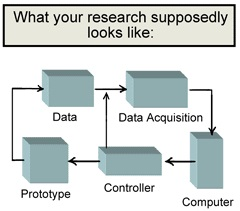
\includegraphics[width=8cm]{figuras/figura-1}}
		}{
			\Fonte{Elaborado pelo autor}
		}	
	\end{figure}
	
\lipsum[11]


\section{Fundamentação Teórica B}
\label{sec:fundamentacao-teorica-b}

Integer non lacinia magna. Aenean tempor lorem tellus, non sodales nisl commodo ut. Proin mattis placerat risus sit amet laoreet \cite{Maia2011}. Praesent sapien arcu, maximus ac fringilla efficitur, vulputate faucibus sem. Donec aliquet velit eros, sit amet elementum dolor pharetra eget. Integer eget mattis libero. Praesent ex velit, pulvinar at massa vel, fermentum dictum mauris. Ut feugiat accumsan augue, et ultrices ipsum euismod vitae

	\begin{figure}[h!]
		\centering
		\Caption{\label{fig:exemplo-2} Maecenas luctus augue odio, sed tincidunt nunc posuere nec}	
		\UECEfig{}{
			\fbox{
\includegraphics[width=8cm]{figuras/figura-2}}
		}{
			\Fonte{Elaborado pelo autor}			
		}	
	\end{figure}

Nunc ac pretium dui. Mauris aliquam dapibus nulla ac mattis. Aenean non tortor volutpat, varius lectus vitae, accumsan nibh. Cras pretium vestibulum enim, id ullamcorper tortor ultrices non. Integer sodales viverra faucibus. Curabitur at dui lacinia, rhoncus lacus at, blandit metus. Integer scelerisque non enim quis ornare.

\lipsum[13]

	\begin{table}[h!]	
		\centering
		\Caption{\label{tab:exemplo-1} Duis faucibus, enim quis tincidunt pellentesque, nisl leo varius nulla, vitae tempus dui mauris ac ante purus lorem}		
		\UECEtab{}{
			\begin{tabular}{cll}
				\toprule
				Ranking & Exon Coverage & Splice Site Support \\
				\midrule \midrule
				E1 & Complete coverage by a single transcript & Both splice sites\\
				E2 & Complete coverage by more than a single transcript & Both splice sites\\
				E3 & Partial coverage & Both splice sites\\
				E4 & Partial coverage & One splice site\\
				E5 & Complete or partial coverage & No splice sites\\
				E6 & No coverage & No splice sites\\
				\bottomrule
			\end{tabular}
		}{
		\Fonte{Elaborado pelo autor}
	}
	\end{table}

Duis faucibus, enim quis tincidunt pellentesque, nisl leo varius nulla, vitae tempus dui mauris ac ante. Quisque purus lorem, pharetra sit amet lobortis eu, vehicula vitae purus. Ut varius, erat nec vehicula elementum, risus est tempus justo, nec vulputate augue leo egestas metus.

	\begin{figure}[h!]
		\centering
		\Caption{\label{fig:exemplo-3} Ut posuere, ex quis sagittis auctor, magna massa euismod felis}	
		\UECEfig{}{
			\fbox{
\includegraphics[width=8cm]{figuras/figura-2}}
		}{
		\Fonte{Elaborado pelo autor}			
	}	
	\end{figure}

\lipsum[14]

	\begin{table}[h!]	
		\centering
		\Caption{\label{tab:exemplo-2} Etiam molestie, nulla a egestas aliquet, velit augue congue metus}		
		\UECEtab{}{
			\begin{tabular}{ccll}
				\toprule
				Quisque & pharetra & tempus & vulputate \\
				\midrule \midrule
				E1 & Complete coverage by a single transcript & Both splice sites\\
				E2 & Complete coverage by more than a single transcript & Both splice sites\\
				E3 & Partial coverage & Both splice sites & Both \\
				E4 & Partial coverage & One splice site & Both \\
				E5 & Complete or partial coverage & No splice sites & Both\\
				E6 & No coverage & No splice sites\\
				\bottomrule
			\end{tabular}
		}{
		\Fonte{Elaborado pelo autor}
	}
	\end{table}
	
Duis faucibus, enim quis tincidunt pellentesque, nisl leo varius nulla, vitae tempus dui mauris ac ante. Quisque purus lorem, pharetra sit amet lobortis eu, vehicula vitae purus.
\acrlong{DATASUS},\acrlong{DNV},\acrlong{DO},\acrlong{ESF},\acrlong{IBGE},\acrlong{MFC},\acrlong{MI},\acrlong{MS},\acrlong{NV},\acrlong{ODM},\acrlong{OI},\acrlong{OMS},\acrlong{ONU},\acrlong{PNI},\acrlong{PSF},\acrlong{RIPSA},\acrlong{RN},\acrlong{SIM},\acrlong{SINASC},\acrlong{SUS},\acrlong{TMI},\acrlong{TMMFC}

\begin{alineascomponto}
	\item Integer non lacinia magna. Aenean tempor lorem tellus, non sodales nisl commodo ut
	\item Proin mattis placerat risus sit amet laoreet. Praesent sapien arcu, maximus ac fringilla efficitur, vulputate faucibus sem. Donec aliquet velit eros, sit amet elementum dolor pharetra eget
	\item Integer eget mattis libero. Praesent ex velit, pulvinar at massa vel, fermentum dictum mauris. Ut feugiat accumsan augue, et ultrices ipsum euismod vitae
	\begin{subalineascomponto}
		\item Integer non lacinia magna. Aenean tempor lorem tellus, non sodales nisl commodo ut
		\item Proin mattis placerat risus sit amet laoreet.
	\end{subalineascomponto}
\end{alineascomponto}
	\chapter{Metodologia}
\label{chap:metodologia}

A metodologia utilizada foi uma simples implementação dos algoritmos utilizando pequenas modificações para o obter o número de comparações e o número de atribuições envolvendo elementos do vetor ao termino da execução.

Cada cenário, variando o número de elementos do vetor e o tipo destes, foi testado ao menos cinco vezes, e os resultados aqui apresentados são uma média dos obtidos durante a realização desta análise.

Os resultados de cada algoritmo nos casos analisados estão explicitados posteriormente nas formas de gráficos e tabelas para uma melhor comparação e exibição.
	\chapter{Algoritmos}
\label{chap:algoritmos}
Os algoritmos aqui utilizados foram os oito primeiros a serem estudados e implementados nas aulas de introdução à ciência da computação II, sendo destes, cinco do tipo simples ou intuitivos, e outros três mais complexos e sofisticados.\\

Abaixo estão um breve resumo de cada algoritmo bem como seus respectivos custos de tempo e memória na notação de O-grande(mais comumente conhecido como Big-O)

Mais a frente os Big-O's dos algoritmos serão verificados com os dados dos testes.

\section{Bubble Sort}
\label{sec:bubble_sort}
O algoritmo de bolha(ordenação por flutuação), mais conhecido como Bubble sort, é o algoritmo de ordenação mais simples de todos, e funciona trocando elementos adjacentes repetidamente de estiverem na ordem errada. Sempre iniciando no primeiro elemento do vetor e indo até o ultimo.
\cite{GeeksforGeeksBubble}

\noindent Pior caso de tempo:O($n^2$)\\
Melhor caso de tempo:O(n)\\
Gasto auxiliar de memoria:O(1)


\section{Bubble Sort com Sentinela}
\label{sec:bubble_sent}
Bubble sort com sentinela é uma otimização do algoritmo citado anteriormente, e funciona adicionando um elemento sentinela para verificar onde houve a primeira interação de troca, assim sabe-se que até aquele ponto o vetor ja esta ordenado e não é necessario verificar todos elementos anteriores a ele.

\noindent Pior caso de tempo:O($n^2$)\\
Melhor caso de tempo:O(n)\\
Gasto auxiliar de memoria:O(1)


\section{Bubble Sort Cocktail Shaker}
\label{sec:cocktail}
Assim como a sentinela, Bubble com coquetel, conhecido também como cocktail sort, é uma variação/otimização do Bubble. Enquanto o tradicional sempre atravessa o vetor da esquerda para direita, o cocktail sort o faz em ambas as direções alternadamente.

\noindent Pior caso de tempo:O($n^2$)\\
Melhor caso de tempo:O(n)\\
Gasto auxiliar de memoria:O(1)


\section{Inserction Sort}
\label{sec:inserction_sort}
Insertion sort, ou ordenação por seleção, é um algoritmo que funciona da maneira que ordenamos cartas na mão, ou seja, pega um elemento e o insere na sua posição correta, arrastando outros para abrir espaço.
\cite{GeeksforGeeksins}

\noindent Pior caso de tempo:O($n^2$)\\
Melhor caso de tempo:O(n)\\
Gasto auxiliar de memoria:O(1)

\section{Selection Sort}
\label{sec:selection_sort}
Selection sort, ou seleção, funciona buscando o menor elemento e o colocando no inicio do vetor não ordenado, assim ele mantém dois subvetores, um de ordenados e outro de não-ordenados.

\noindent Pior caso de tempo:O($n^2$)\\
Melhor caso de tempo:O($n^2$)\\
Gasto auxiliar de memoria:O(1)

\section{Merge Sort}
\label{sec:merge_sort}
Merge Sort, ou intercalação, funciona dividindo o problema em problemas menores, trabalhando com duas funções, uma que divide um vetor em dois menores e uma que intercala dois vetores ordenados em um unico. Como um vetor unitario é sempre ordenado, chamando recursivamente essas funções é possivel ordenar o vetor.

\noindent Pior caso de tempo:O($n\log(n)$)\\
Melhor caso de tempo:O($n\log(n)$)\\
Gasto auxiliar de memoria:O(n)


\section{Heap Sort}
\label{sec:heap_sort}
Heap sort é um algoritmo de ordenação baseado na estrutura binaria de Heap, uma vez com essa estrutura, é semelhante ao selection sort em encontrar o maior elemento e ordenar.

\noindent Pior caso de tempo:O($n\log(n)$)\\
Melhor caso de tempo:O($n\log(n)$)\\
Gasto auxiliar de memoria:O(1)

\section{Quick Sort}
\label{sec:quick_sort}
Quick sort, semelhante ao merge, divide o problema em parcelas menores, pegando um elemento como pivô, faz todos antes dele serem menores, e todos depois dele serem maiores, então repete o processo recursivamente.

\noindent Pior caso de tempo:O($n^2$)\\
Melhor caso de tempo:O($n\log(n)$)\\
Gasto auxiliar de memoria:O(1)
	\chapter{Cenários e Casos teste}
\label{chap:casos_teste}
Para a avaliação dos algoritmos, serão utilizados varios cenários com diversos casos teste.  Primeiramente serão utilizados vetores com $10^k$ elementos, sendo que $2 \leqslant k \leqslant 6$.  Além disso, os elementos desses vetores poderão estar distribuidos de quatro formas diferentes, sendo elas: Completamente aleatória, Quase ordenada, Quase inversamente ordenada e com muitos elementos repetidos.\\

Sendo assim utilizaremos cinco tamanhos de vetores diferentes e quatro distribuições de elementos, totalizando uma quantia de vinte cenários diferentes para ser analisado ao menos cinco vezes em cada um dos oito algoritmos aqui avaliados. \\

Em cada cenário analisado serão registrados dados sobre o número de atribuições e de comparações feitas no vetor, que em seguida serão exibidos nos resultados.
	\chapter{Resultados}
\label{chap:resultados}
Aqui estão os resultados dos testes realizados nos cenários descritos anteriormente.

\section{Bubble Sort}
\label{sec:bubble_sort}
\subsection{Comparações}
\begin{tabular}{|c|c|c|c|c|}
\hline
  & Aleatorio  & Quase Ordenado & Inv. Ordenado & Repetidos \\
\hline
$10^2$ & 9306       & 693            & 9603          & 7722       \\
\hline
$10^3$ & 991008     & 7992           & 993006        & 932067     \\
\hline
$10^4$ & 99140085   & 89991          & 99950004      & 97450254   \\
\hline
$10^5$ & 9906200937 & 999990         & 9999800001    & 9944000559 \\
\hline
$10^6$ & NULL       & NULL           & NULL          & NULL      \\
\hline
\end{tabular}
\subsection{Atribuições}
\begin{tabular}{|c|c|c|c|c|}
\hline
  & Aleatorio  & Quase Ordenado & Inv. Ordenado & Repetidos  \\
  \hline
$10^2$ & 8043       & 423            & 10371         & 7068       \\
\hline
$10^3$ & 762264     & 4224           & 1451094       & 749040     \\
\hline
$10^4$ & 74312238   & 42030          & 149484591     & 75605889   \\
\hline
$10^5$ & 7512681453 & 419583         & 14994853377   & 7473100884 \\
\hline
$10^6$ & NULL       & NULL           & NULL          & NULL      \\
\hline
\end{tabular}

\section{Bubble Sort com Sentinela}
\label{sec:bubble_sent}
\subsection{Comparações}
\begin{tabular}{|c|c|c|c|c|}
\hline
  & Aleatorio  & Quase Ordenado & Inv. Ordenado & Repetidos  \\
  \hline
$10^2$ & 1900       & 1908           & 2059          & 1788       \\
\hline
$10^3$ & 184629     & 254349         & 205795        & 184017     \\
\hline
$10^4$ & 18453753   & 11542759       & 20361953      & 18413768   \\
\hline
$10^5$ & 1842168146 & 3067032680     & 2041626972    & 1843218397 \\
\hline
$10^6$ & NULL       & NULL           & NULL          & NULL      \\
\hline
\end{tabular}
\subsection{Atribuições}
\begin{tabular}{|c|c|c|c|c|}
\hline
  & Aleatorio  & Quase Ordenado & Inv. Ordenado & Repetidos  \\
  \hline
$10^2$ & 4420       & 395            & 5503          & 4030       \\
\hline
$10^3$ & 449876     & 4191           & 610524        & 446453     \\
\hline
$10^4$ & 44947304   & 42026          & 61017085      & 45054740   \\
\hline
$10^5$ & 4510622030 & 419210         & 6124189875    & 4510572345 \\
\hline
$10^6$ & NULL       & NULL           & NULL          & NULL      \\
\hline
\end{tabular}


\section{Bubble Sort Cocktail Shaker}
\label{sec:cocktail}
\subsection{Comparações}
\begin{tabular}{|c|c|c|c|c|}
\hline
  & Aleatorio  & Quase Ordenado & Inv. Ordenado & Repetidos  \\
  \hline
$10^2$ & 5940       & 594            & 7623          & 5940       \\
\hline
$10^3$ & 476523     & 6993           & 980019        & 498501     \\
\hline
$10^4$ & 51444855   & 89991          & 99720027      & 50404959   \\
\hline
$10^5$ & 5028849711 & 899991         & 9997600023    & 5007749922 \\
\hline
$10^6$ & NULL       & NULL           & NULL          & NULL      \\
\hline
\end{tabular}
\subsection{Atribuições}
\begin{tabular}{|c|c|c|c|c|}
\hline
  & Aleatorio  & Quase Ordenado & Inv. Ordenado & Repetidos  \\
  \hline
$10^2$ & 7512       & 435            & 11163         & 7008       \\
\hline
$10^3$ & 720564     & 4050           & 1449165       & 728427     \\
\hline
$10^4$ & 76059789   & 42339          & 149484621     & 74803839   \\
\hline
$10^5$ & 7523061132 & 418974         & 14994848034   & 7492000080 \\
\hline
$10^6$ & NULL       & NULL           & NULL          & NULL      \\
\hline
\end{tabular}

\section{Inserction Sort}
\label{sec:inserction_sort}
\subsection{Comparações}
\begin{tabular}{|c|c|c|c|c|}
\hline
  & Aleatorio  & Quase Ordenado & Inv. Ordenado & Repetidos  \\
  \hline
$10^2$ & 2524       & 135            & 3783          & 2325       \\
\hline
$10^3$ & 250319     & 1400           & 483088        & 248614     \\
\hline
$10^4$ & 24925870   & 14013          & 49828319      & 24947032   \\
\hline
$10^5$ & 2496725225 & 139740         & 4998482442    & 2505577578 \\
\hline
$10^6$ & NULL       & 1402844        & NULL          & NULL      \\
\hline
\end{tabular}
\subsection{Atribuições}
\begin{tabular}{|c|c|c|c|c|}
\hline
  & Aleatorio  & Quase Ordenado & Inv. Ordenado & Repetidos  \\
  \hline
$10^2$ & 2722       & 333            & 3981          & 2523       \\
\hline
$10^3$ & 252317     & 3398           & 485086        & 250612     \\
\hline
$10^4$ & 24945868   & 34011          & 49848317      & 24967030   \\
\hline
$10^5$ & 2496925223 & 339738         & 4998282444    & 2505777576 \\
\hline
$10^6$ & NULL       & 3402842        & NULL          & NULL      \\
\hline
\end{tabular}

\section{Selection Sort}
\label{sec:selection_sort}
\subsection{Comparações}
\begin{tabular}{|c|c|c|c|c|}
\hline
  & Aleatorio  & Quase Ordenado & Inv. Ordenado & Repetidos  \\
  \hline
$10^2$ & 5049       & 5049           & 5049          & 5049       \\
\hline
$10^3$ & 500499     & 500499         & 500499        & 500499     \\
\hline
$10^4$ & 50004999   & 50004999       & 50004999      & 50004999   \\
\hline
$10^5$ & 5000049999 & 5000049999     & 5000049999    & 5000049999 \\
\hline
$10^6$ & NULL       & NULL           & NULL          & NULL      \\
\hline
\end{tabular}
\subsection{Atribuições}
\begin{tabular}{|c|c|c|c|c|}
\hline
  & Aleatorio & Quase Ordenado & Inv. Ordenado & Repetidos \\
  \hline
$10^2$ & 120       & 162            & 99            & 99        \\
\hline
$10^3$ & 1029      & 1623           & 999           & 999       \\
\hline
$10^4$ & 10026     & 16068          & 9999          & 9999      \\
\hline
$10^5$ & 100035    & 161430         & 99999         & 99999     \\
\hline
$10^6$ & NULL      & NULL           & NULL          & NULL     \\
\hline
\end{tabular}

\section{Merge Sort}
\label{sec:merge_sort}
\subsection{Comparações}
\begin{tabular}{|c|c|c|c|c|}
\hline
  & Aleatorio & Quase Ordenado & Inv. Ordenado & Repetidos \\
  \hline
$10^2$ & 536       & 404            & 509           & 530       \\
\hline
$10^3$ & 8603      & 5637           & 7062          & 8562      \\
\hline
$10^4$ & 119562    & 73892          & 87970         & 119582    \\
\hline
$10^5$ & 1526319   & 901733         & 1045371       & 1525984   \\
\hline
$10^6$ & 18560858  & 10638710       & 12086103      & 18561303 \\
\hline
\end{tabular}
\subsection{Atribuições}
\begin{tabular}{|c|c|c|c|c|}
\hline
  & Aleatorio & Quase Ordenado & Inv. Ordenado & Repetidos \\
  \hline
$10^2$ & 1344      & 1344           & 1344          & 1344      \\
\hline
$10^3$ & 19952     & 19952          & 19952         & 19952     \\
\hline
$10^4$ & 267232    & 267232         & 267232        & 267232    \\
\hline
$10^5$ & 3337856   & 3337856        & 3337856       & 3337856   \\
\hline
$10^6$ & 39902848  & 39902848       & 39902848      & 39902848 \\
\hline
\end{tabular}

\section{Heap Sort}
\label{sec:heap_sort}
\subsection{Comparações}
\begin{tabular}{|c|c|c|c|c|}
\hline
  & Aleatorio & Quase Ordenado & Inv. Ordenado & Repetidos \\
  \hline
$10^2$ & 1344      & 1344           & 1344          & 1344      \\
\hline
$10^3$ & 19952     & 19952          & 19952         & 19952     \\
\hline
$10^4$ & 267232    & 267232         & 267232        & 267232    \\
\hline
$10^5$ & 3337856   & 3337856        & 3337856       & 3337856   \\
\hline
$10^6$ & 39902848  & 39902848       & 39902848      & 39902848 \\
\hline
\end{tabular}
\subsection{Atribuições}
\begin{tabular}{|c|c|c|c|c|}
\hline
  & Aleatorio & Quase Ordenado & Inv. Ordenado & Repetidos \\
  \hline
$10^2$ & 1767      & 1884           & 1662          & 1668      \\
\hline
$10^3$ & 27213     & 29025          & 25146         & 27153     \\
\hline
$10^4$ & 372204    & 393885         & 349341        & 372357    \\
\hline
$10^5$ & 4724376   & 4947645        & 4489104       & 4725738   \\
\hline
$10^6$ & 57149343  & 59328996       & 54917466      & 57142287 \\
\hline
\end{tabular}

\section{Quick Sort}
\label{sec:quick_sort}
\subsection{Comparações}
\begin{tabular}{|c|c|c|c|c|}
\hline
  & Aleatorio & Quase Ordenado & Inv. Ordenado & Repetidos \\
  \hline
$10^2$ & 579       & 614            & 531           & 746       \\
\hline
$10^3$ & 10657     & 9943           & 9979          & 12684     \\
\hline
$10^4$ & 146034    & 146075         & 151098        & 170136    \\
\hline
$10^5$ & 1959313   & 1945109        & 1925342       & 2090274   \\
\hline
$10^6$ & 24141819  & 24552279       & 24502073      & 26236616 \\
\hline
\end{tabular}
\subsection{Atribuições}
\begin{tabular}{|c|c|c|c|c|}
\hline
  & Aleatorio & Quase Ordenado & Inv. Ordenado & Repetidos \\
  \hline
$10^2$ & 828       & 678            & 891           & 1085      \\
\hline
$10^3$ & 10816     & 6624           & 10136         & 13097     \\
\hline
$10^4$ & 131680    & 67288          & 102770        & 153558    \\
\hline
$10^5$ & 1538152   & 671870         & 1034338       & 1776925   \\
\hline
$10^6$ & 17707539  & 6718560        & 10345663      & 20002381 \\
\hline
\end{tabular}

	%\chapter{Trabalhos Relacionados}
\label{cap:trabalhos-relacionados}

Integer non lacinia magna. Aenean tempor lorem tellus, non sodales nisl commodo ut. Proin mattis placerat risus sit amet laoreet. Praesent sapien arcu, maximus ac fringilla efficitur, vulputate faucibus sem. Donec aliquet velit eros, sit amet elementum dolor pharetra eget. Integer eget mattis libero

\section{Trabalho Relacionado A}
\label{sec:trabalho-relacionado-a}

\lipsum[10]

	\begin{figure}[h!]
		\centering
		\Caption{\label{fig:exemplo-1} Lorem ipsum dolor sit amet, consectetur adipiscing elit. Suspendisse commodo lectus et augue elementum varius.}	
		\UECEfig{}{
			\fbox{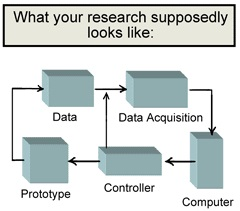
\includegraphics[width=8cm]{figuras/figura-1}}
		}{
			\Fonte{Elaborado pelo autor}
		}	
	\end{figure}
	
\lipsum[11]

\section{Trabalho Relacionado B}
\label{sec:trabalho-relacionado-b}

Integer non lacinia magna. Aenean tempor lorem tellus, non sodales nisl commodo ut. Proin mattis placerat risus sit amet laoreet. Praesent sapien arcu, maximus ac fringilla efficitur, vulputate faucibus sem. Donec aliquet velit eros, sit amet elementum dolor pharetra eget. Integer eget mattis libero. Praesent ex velit, pulvinar at massa vel, fermentum dictum mauris. Ut feugiat accumsan augue, et ultrices ipsum euismod vitae

	\begin{figure}[h!]
		\centering
		\Caption{\label{fig:exemplo-2} Maecenas luctus augue odio, sed tincidunt nunc posuere nec}	
		\UECEfig{}{
			\fbox{
\includegraphics[width=8cm]{figuras/figura-2}}
		}{
			\Fonte{Elaborado pelo autor}			
		}	
	\end{figure}

Nunc ac pretium dui. Mauris aliquam dapibus nulla ac mattis. Aenean non tortor volutpat, varius lectus vitae, accumsan nibh. Cras pretium vestibulum enim, id ullamcorper tortor ultrices non. Integer sodales viverra faucibus. Curabitur at dui lacinia, rhoncus lacus at, blandit metus. Integer scelerisque non enim quis ornare.

	\begin{quadro}[h!]	
		\centering
		\Caption{\label{qua:exemplo-1} Praesent ex velit, pulvinar at massa vel, fermentum dictum mauris. Ut feugiat accumsan augue}		
		\UECEqua{}{
			\begin{tabular}{|c|c|l|l|}
				\hline
				Quisque & pharetra & tempus & vulputate \\
				\hline
				E1 & Complete coverage by a single transcript & Both  & Complete\\
				\hline
				E2 & Complete coverage by more than & Both splice sites & Complete\\
				\hline
				E3 & Partial coverage & Both splice sites & Both \\				
				\hline
			\end{tabular}
		}{
			\Fonte{Elaborado pelo autor}
		}
	\end{quadro}
	
\lipsum[20]

	
	\begin{quadro}[h!]	
		\centering
		\Caption{\label{qua:exemplo-2} Duis faucibus, enim quis tincidunt pellentesque}		
		\UECEqua{}{
			\begin{tabular}{|c|c|}
				\hline
				Quisque & pharetra \\
				\hline
				E1 & Complete coverage by a single transcript \\
				\hline
				E2 & Complete coverage by more than \\
				\hline
				E3 & Partial coverage \\
				\hline
				E4 & Partial coverage \\
				\hline
				E5 & Partial coverage \\
				\hline
				E6 & Partial coverage \\
				\hline
				E7 & Partial coverage \\
				\hline
			\end{tabular}
		}{
			\Fonte{Elaborado pelo autor}
		}
	\end{quadro}

\lipsum[21]

Integer non lacinia magna. Aenean tempor lorem tellus, non sodales nisl commodo ut. Proin mattis placerat risus sit amet laoreet. Praesent sapien arcu, maximus ac fringilla efficitur, vulputate faucibus sem. Donec aliquet velit eros, sit amet elementum dolor pharetra eget. Integer eget mattis libero.
\Gls{ambiguidade}
\Gls{braile}
\Gls{coerencia}
\Gls{dialetos}
\Gls{elipse}
\Gls{locucao-adjetiva}
\Gls{modificadores}
\Gls{paronimos}
\Gls{sintese}
\Gls{borboleta}
	%\chapter{Exemplo de Capítulos e Seções}
\label{chap:exemplo-de-capitulos-e-secoes}

Este capítulo descreve como você deve formatar os títulos do seu trabalho, ensinando também como você deve usá-los. O capítulo deve ser caixa alta, 12pt e com negrito. Para fazer um capítulo, você deve fazer:

\verb!\chapter{Escreva aqui o nome do Capítulo}!

\section{Seção Secundária}
As seções Secundárias deve ser caixa alta, 12pt e sem negrito. Para fazer uma seção Secundária, você deve fazer:

\verb!\section{Escreva aqui o nome da seção}!

\subsection{Seção Terciária}
As seções Terciárias deve ser caixa alta e baixa, 12pt e com negrito. Para fazer uma seção Terciária, você deve fazer:

\verb!\subsection{Escreva aqui o nome da seção}!

\subsubsection{Seção Quaternária}
As seções Quaternárias deve ser caixa alta e baixa, 12pt e sem negrito. Para fazer uma seção Quaternária, você deve fazer:

\verb!\subsubsection{Escreva aqui o nome da seção}!

\subsubsubsection{Seção Quinária}
As seções Quinárias deve ser caixa alta e baixa, 12pt e com itálico. Para fazer uma seção Quinária, você deve fazer:

\verb!\subsubsubsection{Escreva aqui o nome da seção}!
	\chapter{Conclusão}
\label{chap:conclusao}

Como pode-se verificar com os testes realizados, não existe um algoritmo perfeito para todos os possiveis cenários, até mesmo os mais sofisticados e complexos são ultrapassados pelos simples em alguns casos específicos.

Apesar deste resultado ambíguo, algumas ressalvas são importantes: Em um caso geral com vetores de tamanhos maiores $10^5$ a eficácia do Merge Sort, Heap Sort e Quick Sort sobre os demais é gigantesca, deixando extremamente frisado a diferença de um Big-O de O($n^2$) para o O($n\log(n))$ desses algoritmos.

Dissertando mais especificamente sobre os resultos obtidos por cada algoritmo, primeiramente, sobre os algoritmos intuitivos:

\begin{itemize}
   \item Bubble sort e suas otimizações, bubble com sentinela e cocktail sort, todos funcionam de maneira semelhante, apesar de os dois ultimos trabalharem mais eficientemente, o resultado final não varia muito. Funciona muito bem para vetores quase ordenados, e não muito bem nos demais, possui um declinio muito grande na eficiencia com o aumento do vetor.
   
   \item O inserction sort em um caso geral possui em desempenho semelhante ao bubble, porém no caso de vetor quase ordenado possui o melhor desempenho entre todos aqui avaliados.
   
   \item Selection sort possui a mesma ordem que os demais intuitivos, porém possui o pior desempenho entre eles, para todos os casos. Seu unico ponto positivo é o baixo número de atribuições.
   
\end{itemize}
   
Por fim, os algoritmos mais sofisticados e seus pontos positivos e negativos:
\begin{itemize}
   \item Merge sort, o primeiro dos complexos aqui avaliados, possui O($n\log(n)$) sendo muito mais eficiente que os anteriores e possuindo um desempenho constante para todos os casos, se destacando um pouco mais no caso quase ordenado. Seu principal ponto negativo, apesar de não ser exibido pelos testes, é seu gasto de memória ser O(n), contra O(1) dos demais algoritmos.
   
   \item Heap sort, organiza o vetor no mesmo Big O que o merge, porém sem o ponto negativo de gasto extra de espaço. Algoritmo muito eficiente, tendo apenas um grande defeito, que é ser contante no tempo independente do tipo de vetor, o gasto é o mesmo.
   
   \item E por ultimo, quick sort, assim como os demais aqui avaliados, possui um desempelho excelente em seu caso geral, não necessitando de espaço extra como o merge, e se beneficiando mais da situação do vetor que o heap. Possui um pouco de dificuldade em vetores com muitos elementos repetidos, porém seu defeito esta no pior caso, que apesar de raro, o torna um algoritmo com complexidade de tempo O($n^2$).
 \end{itemize}
	%\chapter{CRONOGRAMA}
\label{ap:modelo-de-capa}

\center

\begin{enumerate}
\item Pesquisa bibliográfica
\item Estudo e preparação do estado da arte
\item Programação e/ou experimentação e/ou simulação
\item Análise dos resultados
\item Redação da dissertação
\item Apresentação do trabalho
\end{enumerate}

\begin{table}[h]
	\centering
	\begin{tabular}{|l|l|l|l|l|}
	\hline
	\multicolumn{1}{|c|}{} &
	\multicolumn{4}{|c|}{MESES} \\
	\hline
	\multicolumn{1}{|c|}{ETAPAS} &
	\multicolumn{1}{c|}{Mês 1} &
	\multicolumn{1}{c|}{Mês 2} &
	\multicolumn{1}{c|}{Mês 3} &
	\multicolumn{1}{c|}{Mês 4} \\
	\hline
        \multicolumn{1}{|c|}{1} &
        \cellcolor[gray]{0.8}\color{black} &
        \multicolumn{1}{c|}{} &
        \multicolumn{1}{c|}{} &
        \multicolumn{1}{c|}{} \\
	\hline
        \multicolumn{1}{|c|}{2} &
        \cellcolor[gray]{0.8}\color{black} &
        \multicolumn{1}{c|}{} &
        \multicolumn{1}{c|}{} &
        \multicolumn{1}{c|}{} \\
	\hline
        \multicolumn{1}{|c|}{3} &
        \multicolumn{1}{c|}{} &
        \cellcolor[gray]{0.8}\color{black} &
        \multicolumn{1}{c|}{} &
        \multicolumn{1}{c|}{} \\
	\hline
        \multicolumn{1}{|c|}{4} &
        \multicolumn{1}{c|}{} &
        \multicolumn{1}{c|}{} &
        \cellcolor[gray]{0.8}\color{black} &
        \multicolumn{1}{c|}{} \\
	\hline
        \multicolumn{1}{|c|}{5} &
        \multicolumn{1}{c|}{} &
        \multicolumn{1}{c|}{} &
        \multicolumn{1}{c|}{} &
        \cellcolor[gray]{0.8}\color{black} \\
	\hline
        \multicolumn{1}{|c|}{6} &
        \multicolumn{1}{c|}{} &
        \multicolumn{1}{c|}{} &
        \multicolumn{1}{c|}{} &
        \cellcolor[gray]{0.8}\color{black} \\
%	\hline
%        \multicolumn{1}{|c|}{7} &
%        \multicolumn{1}{c|}{} &
%        \multicolumn{1}{c|}{} &
%        \multicolumn{1}{c|}{} &
%        \multicolumn{1}{c|}{} \\
	\hline
	\end{tabular}
\end{table}
	
	%Elementos pós-textuais	
	\bibliography{elementos-pos-textuais/referencias}
	%\imprimirglossario	
	%\imprimirapendices
		% Adicione aqui os apendices do seu trabalho
		%\chapter{CRONOGRAMA}
\label{ap:modelo-de-capa}

\center

\begin{enumerate}
\item Pesquisa bibliográfica
\item Estudo e preparação do estado da arte
\item Programação e/ou experimentação e/ou simulação
\item Análise dos resultados
\item Redação da dissertação
\item Apresentação do trabalho
\end{enumerate}

\begin{table}[h]
	\centering
	\begin{tabular}{|l|l|l|l|l|}
	\hline
	\multicolumn{1}{|c|}{} &
	\multicolumn{4}{|c|}{MESES} \\
	\hline
	\multicolumn{1}{|c|}{ETAPAS} &
	\multicolumn{1}{c|}{Mês 1} &
	\multicolumn{1}{c|}{Mês 2} &
	\multicolumn{1}{c|}{Mês 3} &
	\multicolumn{1}{c|}{Mês 4} \\
	\hline
        \multicolumn{1}{|c|}{1} &
        \cellcolor[gray]{0.8}\color{black} &
        \multicolumn{1}{c|}{} &
        \multicolumn{1}{c|}{} &
        \multicolumn{1}{c|}{} \\
	\hline
        \multicolumn{1}{|c|}{2} &
        \cellcolor[gray]{0.8}\color{black} &
        \multicolumn{1}{c|}{} &
        \multicolumn{1}{c|}{} &
        \multicolumn{1}{c|}{} \\
	\hline
        \multicolumn{1}{|c|}{3} &
        \multicolumn{1}{c|}{} &
        \cellcolor[gray]{0.8}\color{black} &
        \multicolumn{1}{c|}{} &
        \multicolumn{1}{c|}{} \\
	\hline
        \multicolumn{1}{|c|}{4} &
        \multicolumn{1}{c|}{} &
        \multicolumn{1}{c|}{} &
        \cellcolor[gray]{0.8}\color{black} &
        \multicolumn{1}{c|}{} \\
	\hline
        \multicolumn{1}{|c|}{5} &
        \multicolumn{1}{c|}{} &
        \multicolumn{1}{c|}{} &
        \multicolumn{1}{c|}{} &
        \cellcolor[gray]{0.8}\color{black} \\
	\hline
        \multicolumn{1}{|c|}{6} &
        \multicolumn{1}{c|}{} &
        \multicolumn{1}{c|}{} &
        \multicolumn{1}{c|}{} &
        \cellcolor[gray]{0.8}\color{black} \\
%	\hline
%        \multicolumn{1}{|c|}{7} &
%        \multicolumn{1}{c|}{} &
%        \multicolumn{1}{c|}{} &
%        \multicolumn{1}{c|}{} &
%        \multicolumn{1}{c|}{} \\
	\hline
	\end{tabular}
\end{table}
		%\apendice{Modelo de Capa}
\label{ap:modelo-de-capa}

\lipsum[1]

		%\apendice{Termo de Fiel Depositário}
\label{ap:termo-de-fiel-depositario}

\noindent \textbf{Pesquisa:} ANÁLISE DA MORTALIDADE INFANTIL COM MALFORMAÇÕES CONGÊNITAS.

\noindent Pelo presente instrumento que atende às exigências legais, a Sra. Maria Consuelo Martins Saraiva, ``fiel depositário'' com o cargo de Secretária Municipal de Saúde de Iracema, após ter tomado conhecimento do protocolo de pesquisa intitulado: ANÁLISE DA MORTALIDADE INFANTIL COM MALFORMAÇÕES CONGÊNITAS. Analisando a repercussão desse estudo no contexto da saúde pública e epidemiologia, autoriza Karla Maria da Silva Lima, enfermeira, aluna do Curso de Mestrado Acadêmico em Enfermagem da Universidade Estadual do Ceará (UECE), sob orientação do Prof. Dr. José Maria de Castro, da UECE, ter acesso aos bancos de dados do Sistema de Informação sobre Nascidos Vivos e do Sistema de Informação sobre Mortalidade da Secretaria Municipal de Saúde de Iracema, objeto deste estudo, e que se encontram sob sua total responsabilidade. Fica claro que o Fiel Depositário pode a qualquer momento retirar sua AUTORIZAÇÃO e ciente de que todas as informações prestadas tornar-se-ão confidenciais e guardadas por força de sigilo profissional, assegurando que os dados obtidos da pesquisa serão somente utilizados para estudo.	
	%\imprimiranexos
		% Adicione aqui os anexos do seu trabalho
		%\anexo{Dinâmica das classes sociais}
\label{an:dinamica-das-classes-sociais}

\index{AAA}
	%\imprimirindice

\end{document}